This chapter presents the results of the main experiment and is structured as follows. At first, we describe the design of the experiment. This is done by discussing the different groups that are tested against each other, the algorithm that is used to obtain the decomposition, and the input projects used for experimentation. After the experimental design, we present the results of the experiment. 

\section{Experimental design}
To understand the effect of the utilised information stream on the microservice decomposition, we make seven different decompositions of the system with our proposed tool. Each decomposition is constructed with a unique stream of data. The different input data streams are listed below. Each input stream gets an identifier of three letters based on the data it incorporates. The first letter $S$ represents static data, the second one $L$ lexical data, and the third one $D$ dynamic data. When a data source is not included, the letter $X$ is given.

\begin{itemize}
    \item[$SXX$] \textbf{Static.} The candidate microservices that are obtained by only considering static dependencies as input.
    \item[$XLX$] \textbf{Lexical.} The decompositions obtained when only considering semantic information. This means the graph only consists of semantic edges.
    \item[$XXD$] \textbf{Dynamic.} The decompositions constructed with only dynamic dependencies.
    \item[$SXD$] \textbf{Static and dynamic.} These decompositions are constructed with static and dynamic data as input. This means that both the static and dynamic edges are given in the graph. When an edge has both a static and a dynamic dependency, the edge weights are combined by taking 50 percent of each weight.
    \item[$SLX$] \textbf{Static and semantic.} The fifth group of decompositions combines static with semantic information as input. The edges are combined the same way as before.
    \item[$XLD$] \textbf{Dynamic and semantic.} These decompositions are constructed with dynamic and semantic information as input.
    \item[$SLD$] \textbf{Static, dynamic and semantic.} This group of decompositions takes all three streams of data as input. This means, the edges in the graph can either represent a static, semantic or dynamic edge, or a combination of those. When an edge is combined, each information source counts for 33 percent. This way the maximum weight of the combined edge can never exceed a value of 1. 
\end{itemize}

\subsection{Algorithm and parameters}
The aim of this thesis is the understand how the quality of the microservices changes when different streams of data are used. To make sure the change in the quality of the decomposition is caused by the selected stream of data, it is important to understand how the clustering algorithm influences the result. In the next section, we therefore analyse the impact of the clustering algorithm on the quality of the resulting decomposition.

\subsubsection{The effect of the clustering algorithm}
To measure the effect of the clustering algorithm, we apply the three clustering algorithms selected in Section \ref{step3:graphs} on three graphs created with static, semantic and the two combined as input. Since the Clauset-Newman-Moore algorithm gave strange results for the CHM and CHD metric, we incorporated a fourth clustering algorithm called Label Propogation. The Label Propogation algorithm (LPA), introduced by \citeauthor{raghavan2007near} \cite{raghavan2007near}, is hierarchical based and has an agglomerative character.\par
The three graphs are constructed for two monolithic projects of different sizes. We then observe the change in the results in terms of CHD, CHM, SMQ, and CMQ. When the change in the results are the same direction (all positive or negative) for each clustering algorithm, we assume the algorithm does not affect the change of the results. The results of this experiment are given in Table \ref{tab:effect_algorithm}. \par

\begin{table}[h]
    \footnotesize
    \caption[The effect of the clustering algorithm.]{Results on the effect of the clustering algorithm.}\label{tab:effect_algorithm}
    %This table gives the results of four clustering algorithms applied on three experiments. The best results for Louvain were found with a resolution value of 1. Girvan-Newman gave the best resolution with a cutting value of 5. The last row shows the most frequent change in the results when comparing it to previous column. $>$ indicates the value of the former is bigger than the latter and $<$ vice versa. The number in the brackets shows how many times the change happens. When the change is equal, the $=$ symbol is used. 
    \begin{adjustbox}{center}
    \begin{tabular}{>{\raggedright}m{20pt}>{\raggedright}m{75pt}>{\raggedright}m{18pt}>{\raggedright}m{18pt}>{\raggedright}m{18pt}>{\raggedright}m{18pt}>{\raggedright}m{18pt}>{\raggedright}m{18pt}>{\raggedright}m{18pt}>{\raggedright}m{18pt}>{\raggedright}m{18pt}>{\raggedright}m{18pt}>{\raggedright}m{18pt}>{\raggedright\arraybackslash}m{18pt}}
        \toprule
        Mono
        & Algo
        & \multicolumn{3}{c}{CHM} 
        & \multicolumn{3}{c}{CHD}
        & \multicolumn{3}{c}{SMQ}
        & \multicolumn{3}{c}{CMQ} \\
        & & $SXX$ & $XLX$ & $SLX$ & $SXX$ & $XLX$ & $SLX$ & $SXX$ & $XLX$ & $SLX$ & $SXX$ & $XLX$ & $SLX$ \\
        \midrule
        \multirow{4}*{$M_2$} & Louvain & 0.667 & 0.609 & 0.750 & 0.701 & 0.742 & 0.813 & 0.124 & 0.033 & 0.048 & 0.060 & 0.226 & 0.137 \\
        & Girvan-Newman & 0.498 & 0.586 & 0.619 & 0.562 & 0.753 & 0.754 & 0.092 & 0.021 & 0.012 & 0.039 & 0.199 & 0.197 \\
        & Clauset & 0.440 & 0 & 0 & 0.519 & 0 & 0 & 0.090 & 0.009 & 0.019 & 0.033 & 0.050 & 0.043 \\
        & LPA & 0.667 & 0.620 & 0.657 & 0.695 & 0.745 & 0.783 & 0.170 & 0.039 & 0.056 & 0.081 & 0.254 & 0.188 \\
        \midrule
        \midrule
        & Change & - & (3)$>$ & (3)$<$ & - & (3)$<$ & (3)$<$ & - & (4)$>$ & (4)$<$ & - & (4)$<$ & (4)$>$ \\
        \midrule
        \multirow{4}*{$M_4$} & Louvain & 0.762 & 0.600 & 0.661 & 0.792 & 0.665 & 0.708 & 0.180 & 0.032 & 0.039 & 0.160 & 0.225 & 0.221 \\
        & Girvan-Newman & 0.619 & 0.788 & 0.812 & 0.613 & 0.846 & 0.886 & 0.160 & 0.015 & 0.010 & 0.148 & 0.266 & 0.199 \\
        & Clauset & 1 & 0 & 0 & 1 & 0 & 0 & 0.204 & 0.009 & 0.012 & 0.202 & 0.083 & 0.079 \\
        & LPA & 0.799 & 0.712 & 0.814 & 0.792 & 0.733 & 0.798 & 0.211 & 0.069 & 0.076 & 0.162 & 0.232 & 0.228 \\
        \midrule
        \midrule
        & Change & - & (3)$>$ & (3)$<$ & - & (3)$>$ & (3)$<$ & - & (4)$>$ & (3)$<$ & - & (3)$<$ & (4)$>$ \\
        \bottomrule
    \end{tabular}
    \end{adjustbox}
\end{table}

The Louvain algorithm is tested with different resolution parameters ranging between the values 0.3 and 1. The resolution value with the best performance is chosen and given in the table. The same applies for the input parameter for the Girvan-Newman algorithm. We tried different cutting values ranging between 0 and 5 and selected the best performing one. \par
The row under the double line shows the most frequent type of change that occurs in the results when comparing it to previous column. The greater than ($>$) symbol indicates that the value of the former is bigger than the latter and the less than ($<$) symbol the opposite. The number in the brackets shows how many times the change happens. When the change is equal, the $=$ symbol is used. \par
The table above (Table \ref{tab:effect_algorithm}) shows that most of the times the change in the results is the same for the algorithms. From the 106 observed changes, 96 appear to have the same direction. This means that 91 percent of the changes are the same regardless of the clustering algorithm. For this reason, we decided to select only one algorithm for the main experiment. We decided to go for the Louvain algorithm with a resolution parameter of 1, as it gave the most satisfying and consistent results. For the tf-idf threshold value, we selected a value of 0.05. Increasing this value results in a lower coverage of the semantic constructed graph. A value of 0.05 gave satisfying results during verification and will therefore be used in the remaining experiment.

\subsection{Project collection}
Table \ref{tab:projects_statistics} shows the projects that are used for experimentation. Each monolithic project $M$ is enriched with some descriptive statistics, such as the source lines of code (SLOC) and the number of classes, modules, methods and functions. Below, we give a short description of each project. The projects are ordered by its complexity (in terms of SLOC), starting with the smallest project.

\begin{enumerate}
    \item[$M_1$]\textbf{PyPystore.} PyPetstore\footnote{\href{https://github.com/larsvasseldonk/PyPetstore}{https://github.com/larsvasseldonk/PyPetstore}} is a minimal working command-line tool, inspired by JPetstore, that supports the process of selling pets. PyPetstore serves as an 'toy' example in which we can verify the working of our proposed technique.
    \item[$M_2$] \textbf{twitter} The twitter\footnote{\href{https://github.com/python-twitter-tools/twitter}{https://github.com/python-twitter-tools/twitter}} project includes a set of Python tools such as a Twitter API, command-line tool, and IRC bot. The command-line tool allows you to, e.g., get friends' tweets and setting your own tweet. The IRC bot announces Twitter updates to an IRC channel. 
    \item[$M_3$] \textbf{ChatterBot.} ChatterBot\footnote{\href{https://github.com/gunthercox/ChatterBot}{https://github.com/gunthercox/ChatterBot}} is a machine-learning based conversational dialog engine build in Python which makes it possible to generate responses based on collections of known conversations.
    \item[$M_4$] \textbf{asreview.} ASReview\footnote{\href{https://github.com/asreview/asreview}{https://github.com/asreview/asreview}} (Active learning for Systematic Reviews) implements machine learning algorithms that interactively query the researcher. The project is developed and maintained by Utrecht University and is designed to accelerate the step of screening abstracts and titles with a minimum of papers to be read by a human.
    \item[$M_5$] \textbf{beets.} Beets\footnote{\href{https://github.com/beetbox/beets}{https://github.com/beetbox/beets}} is the media library management system for obsessive music geeks. The project enables users manage music collections by, e.g., automatically improving metadata. It also provides a set of tools to manipulate and access music.
    \item[$M_6$] \textbf{Picard.} MusicBrainz Picard\footnote{\href{https://github.com/metabrainz/picard}{https://github.com/metabrainz/picard}} is a cross-platform (Linux/Mac OS X/Windows) application written in Python and is the official MusicBrainz tagger. The project's public facing website is \href{https://picard.musicbrainz.org/}{https://picard.musicbrainz.org/}. MusicBrainz is an open music encyclopedia that collects music metadata and makes it available to the public.
    \item[$M_7$] \textbf{mu.} Mu\footnote{\href{https://github.com/mu-editor/mu}{https://github.com/mu-editor/mu}} is a simple code editor for beginner programmers based on extensive feedback from teachers and learners. The project's public facing website is \href{https://codewith.mu/}{https://codewith.mu/}.
\end{enumerate}

\begin{table}[h]
    \small
    \caption[Python project for experimentation]{Python projects for experimentation. For each project, we have collected the number of modules, classes, methods and functions available in the code base. The SLOC resembles the number of Python lines of code. }\label{tab:projects_statistics}
    \begin{tabular}{>{\raggedright}m{60pt}>{\raggedright}m{35pt}>{\raggedright}m{30pt}>{\raggedright}m{35pt}>{\raggedright}m{40pt}>{\raggedright\arraybackslash}m{50pt}}
        \toprule
        Project & SLOC & Files & Classes & Methods & Functions\\
        \midrule
        PyPetstore & 556 & 8 & 5 & 40 & 18\\
        \midrule
        twitter & 3510 & 17 & 66 & 117 & 64 \\
        \midrule
        Chatterbot & 10297 & 39 & 46 & 124 & 30 \\
        \midrule
        asreview & 11947 & 101 & 58 & 256 & 280 \\
        \midrule
        beets & 44829 & 29 & 134 & 575 & 290 \\
        \midrule
        picard & 62559 & 196 & 352 & 2027 & 465 \\
        \midrule
        mu & 78628 & 45 & 71 & 524 & 70 \\
        \bottomrule
    \end{tabular}  
\end{table}

\section{Results}
Each of the aforementioned project is analysed with our multi-view clustering tool. Out of this tool, a set of static, semantic and dynamic edges derives. These edges are then used to construct seven different graphs. Subsequently, the Louvain algorithm is used to find communities (microservices) in the graph such that nodes within a community are highly connected, and nodes between communities have low connections. The nodes in the graph represent top-level code fragments, where each top-level code fragment can either be a module (with its inner functions) or a class (with its inner methods). The quality of the candidate micoservices are then measured with the functional independence and modularity metrics. To understand what the effect of the input data is, we rigorously test if the quality of a decomposition resulting from a given information stream outperforms another. We use the paired t-test to validate whether the quality of two decomposition made with different streams of information are significantly different. Two groups are significantly different when the paired t-test results in a p-value lower than 0.05. In the next sections, we give the results of the experiment for each quality metric. \par

\subsection{Functional independence}
As described in Section \ref{s:quality_computation}, we measure the quality of the resulting candidate microservices in terms of its functional independence. The functional independence is measured according to four metrics, namely, CHD, CHM, IFN and OPN. Table \ref{tab:results_chd}, \ref{tab:results_chm}, \ref{tab:results_ifn}, and \ref{tab:results_opn} show the result of each metric respectively when applying our tool with different input data. The last row of each table gives the mean value of each experiment. The experiment with the best mean score is marked with a grey cell colour.

\paragraph{Cohesion at domain level} The CHD metrics aims to measure the cohesiveness of services at domain level. The higher the CHD, the more functional cohesive the services are \cite{jin2018functionality}. Table \ref{tab:results_chd} shows the CHD scores for each input information stream. On average, the highest score for CHD is achieved when all three information streams are used for the decomposition ($SLD$). This makes sense since the algorithm has more information to make a suitable decomposition. However, it is not always that more information results in higher CHD scores. When static and dynamic is combined as input ($SXD$), the average CHD score lies somewhere between the two CHD scores achieved when both streams are used individually ($SXX$ and $XXD$). However, this is on average. When we look at the data again, we note that bigger applications ($M_5$, $M_6$, and $M_7$) always get a higher CHD score when static and dynamic data are combined as input than when they are used individually. The same pattern applies when static and lexical data streams ($SLX$) are combined as input. On average, this again results in a higher CHD score (0.615) than when only static (0.544) or only lexical (0.598) are used. This pattern is in line with our expectations that more views of the system result in a higher quality of the decomposition. When lexical and dynamic information ($XLD$) are combined as input, we see a small decrease in the average CHD score (0.591) compared to the average CHD score achieved when lexical data ($XLX$) is used only (0.598). However, the score is still higher than only using dynamic information ($XXD$) as input (0.537). Each combination of input streams is tested with a paired t-test, but none of them are significantly different. 

\begin{table}[h]
    \footnotesize
    \caption{Results of the main experiment in terms of CHD.}\label{tab:results_chd}
    \begin{adjustbox}{center}
    \begin{tabular}{>{\raggedright}m{20pt}>{\raggedright}m{20pt}>{\raggedright}m{25pt}>{\raggedright}m{20pt}>{\raggedright}m{20pt}>{\raggedright}m{25pt}>{\raggedright}m{20pt}>{\raggedright\arraybackslash}m{20pt}}
        \toprule
        Mono
        & \multicolumn{7}{c}{CHD}\\
        & $SXX$ & $XLX$ & $XXD$ & $SXD$ & $SLX$ & $XLD$ & $SLD$\\
        \midrule
        $M_1$ 
        & 0.511 & 0.479 & 0.528 & 0.479 & 0.417 & 0.479 & 0.479\\
        $M_2$ 
        & 0.375 & 0.641 & 0.633 & 0.375 & 0.595 & 0.624 & 0.632 \\
        $M_3$ 
        & 0.500 & 0.494 & 0.567 & 0.457 & 0.557 & 0.562 & 0.485 \\
        $M_4$ 
        & 0.755 & 0.688 & 0.579 & 0.655 & 0.693 & 0.681 & 0.706 \\
        $M_5$ 
        & 0.452 & 0.496 & 0.336 & 0.506 & 0.506 & 0.451 & 0.509 \\
        $M_6$ 
        & 0.770 & 0.746 & 0.631 & 0.810 & 0.748 & 0.734 & 0.771 \\
        $M_7$ 
        & 0.448 & 0.642 & 0.484 & 0.501 & 0.791 & 0.605 & 0.786 \\
        \midrule
        \midrule
        $avg$ & 0.544 & 0.598 & 0.537 & 0.540 & 0.615 & 0.591 & \cellcolor{CellGray}0.624\\
        \bottomrule
    \end{tabular}
    \end{adjustbox}
\end{table}

% Projects are alphabetically ordered
% IN: IN1 & IN2 & IN3 & IN4 & IN5 & IN6 & IN7

% M1 PyPetstore
% CHM: 0.756 & 0.305 & 0.369 & 0.250 & 0.667 & 0.250 & 0.250
% CHD: 0.511 & 0.044 & 0.528 & 0.479 & 0.444 & 0.479 & 0.479
% IFN: 1.25 & 4 & 2 & 1.333 & 1 & 1.333 & 1.333
% OPN: 15 & 18 & 19 & 10 & 7 & 10 & 10
% SMQ: 0.125 & -0.094 & 0.167 & 0.211 & 0.146 & 0.211 & 0.211
% CMQ: 0.125 & 0.062 & 0.086 & 0.127 & -0.042 & 0.125 & 0.125
% CF: 0.655 & 0.793 & 0.653 & 0.947 & 0.773 & 0.838 & 0.88
% Coverage: 0.667 & 0.667 & 1 & 0.667 & 1 & 1

% M2 twitter
% CHM: 0.293 & 0.721 & 0.704 & 0.486 & 0.755 & 0.772 & 0.766
% CHD: 0.5 & 0.661 & 0.667 & 0.636 & 0.789 & 0.745 & 0.773
% IFN: 2 & 3.625 & 4.5 & 3.667 & 2.714 & 3.875 & 3.667
% OPN: 20 & 53 & 16 & 26 & 32 & 49 & 37
% SMQ: 0.149 & 0.022 & 0.11 & 0.142 & 0.052 & 0.041 & 0.052
% CMQ: 0.114 & 0.198 & 0.077 & 0.09 & 0.176 & 0.207 & 0.146
% CF: 0.684 & 0.774 & 0.628 & 0.561 & 0.744 & 0.881 & 0.871
% Coverage: 0.615 & 0.910 & 0.423 & 0.756 & 0.962 & 0.987 & 0.987

% M3 ChatterBot
% CHM: 0.752 & 0.516 & 0.673 & 0.563 & 0.568 & 0.489 & 0.561
% CHD: 0.767 & 0.409 & 0.517 & 0.463 & 0.529 & 0.408 & 0.513
% IFN: 2.5 & 4 & 2.25 & 2.857 & 3.5 & 4.6 & 4
% OPN: 28 & 46 & 20 & 43 & 48 & 58 & 42
% SMQ: 0.190 & 0.030 & 0.138 & 0.149 & 0.069 & 0.038 & 0.050
% CMQ: 0.044 & 0.233 & 0.030 & 0.027 & 0.126 & 0.136 & 0.108
% Coverage: 0.449 & 0.878 & 0.653 & 0.714 & 0.898 & 0.959 & 0.980

% M4 asreview
% CHM: 0.747 & 0.668 & 0.696 & 0.707 & 0.725 & 0.669 & 0.661
% CHD: 0.730 & 0.612 & 0.599 & 0.665 & 0.685 & 0.627 & 0.630
% IFN: 4.5 & 9.6 & 4.833 & 4.125 & 7.8 & 8.333 & 8.8
% OPN: 55 & 112 & 73 & 81 & 80 & 113 & 90
% SMQ: 0.179 & 0.033 & 0.175 & 0.192 & 0.038 & 0.034 & 0.039
% CMQ: 0.169 & 0.224 & 0.054 & 0.133 & 0.223 & 0.203 & 0.15
% Coverage: 0.732 & 0.961 & 0.661 & 0.913 & 0.984 & 0.992 & 1

% M5 beets
% CHM: 0.627 & 0.653 & 0.570 & 0.604 & 0.649 & 0.644 & 0.622
% CHD: 0.365 & 0.527 & 0.450 & 0.510 & 0.528 & 0.514 & 0.481
% IFN: 4.667 & 14.8 & 7.167 & 6.667 & 12.667 & 14.4 & 12.167
% OPN: 100 & 234 & 162 & 127 & 238 & 215 & 225
% SMQ: 0.152 & 0.02 & 0.082 & 0.128 & 0.022 & 0.023 & 0.03
% CMQ: 0.141 & 0.165 & 0.045 & 0.106 & 0.173 & 0.167 & 0.167
% Coverage: 0.645 & 1 & 0.671 & 0.865 & 1 & 1 & 1

% M6 picard
% CHM: 0.799 & 0.712 & 0.667 & 0.799 & 0.690 & 0.735 & 0.759
% CHD: 0.871 & 0.784 & 0.757 & 0.851 & 0.759 & 0.812 & 0.806
% IFN: 4.688 & 23.5 & 3.667 & 5.933 & 21.25 & 26 & 18.5
% OPN: 112 & 357 & 109 & 138 & 321 & 332 & 267
% SMQ: 0.139 & 0.009 & 0.153 & 0.130 & 0.016 & 0.008 & 0.024
% CMQ: 0.133 & 0.155 & 0.114 & 0.113 & 0.143 & 0.146 & 0.160
% Coverage: 0.69 & 0.998 & 0.4 & 0.841 & 1 & 0.998 & 1

% M7 mu
% CHM: 0.720 & 0.699 & 0.537 & 0.802 & 0.737 & 0.739 & 0.782
% CHD: 0.472 & 0.564 & 0.359 & 0.584 & 0.517 & 0.624 & 0.546
% IFN: 2.143 & 8.8 & 2.4 & 2.556 & 4.4 & 6.667 & 3.8
% OPN: 44 & 121 & 30 & 58 & 55 & 87 & 48
% SMQ: 0.154 & 0.021 & 0.132 & 0.157 & 0.084 & 0.036 & 0.085
% CMQ: 0.115 & 0.119 & 0.032 & 0.097 & 0.110 & 0.124 & 0.111
% Coverage: 0.733 & 0.933 & 0.544 & 0.833 & 0.944 & 0.989 & 1


% Data per group (experiment) for statistical test

% PICARD NOT YET INCLUDED
% CHD
% ex1: 0.511, 0.500, 0.767, 0.730, 0.365, 0.871, 0.472
% ex2: 0.044, 0.661, 0.409, 0.612, 0.527, 0.784, 0.564
% ex3: 0.528, 0.667, 0.517, 0.599, 0.450, 0.757, 0.359
% ex4: 0.479, 0.636, 0.463, 0.665, 0.510, 0.851, 0.584
% ex5: 0.444, 0.789, 0.529, 0.685, 0.528, 0.759, 0.517
% ex6: 0.479, 0.745, 0.408, 0.627, 0.514, 0.812, 0.624
% ex7: 0.479, 0.773, 0.513, 0.630, 0.481, 0.806, 0.546

% CHM
% ex1: 0.756, 0.293, 0.752, 0.747, 0.627, 0.799, 0.720
% ex2: 0.305, 0.721, 0.516, 0.668, 0.653, 0.712, 0.699
% ex3: 0.369, 0.704, 0.673, 0.696, 0.570, 0.667, 0.537
% ex4: 0.250, 0.486, 0.563, 0.707, 0.604, 0.799, 0.802
% ex5: 0.667, 0.755, 0.568, 0.725, 0.649, 0.690, 0.737
% ex6: 0.250, 0.772, 0.489, 0.669, 0.644, 0.735, 0.739
% ex7: 0.250, 0.766, 0.561, 0.661, 0.622, 0.759, 0.782

% IFN
% ex1: 1.25, 2, 2.5, 4.5, 4.667, 4.688, 2.143
% ex2: 4, 3.625, 4, 9.6, 14.8, 23.5, 8.8
% ex3: 2, 4.5, 2.25, 4.833, 7.167, 3.667, 2.4
% ex4: 1.333, 3.667, 2.857, 4.125, 6.667, 5.933, 2.556
% ex5: 1, 2.714, 3.5, 7.8, 12.667, 21.25, 4.4
% ex6: 1.333, 3.875, 4.6, 8.333, 14.4, 26, 6.667
% ex7: 1.333, 3.667, 4, 8.8, 12.167, 18.5, 3.8

% OPN
% ex1: 15, 20, 28, 55, 100, 112, 44
% ex2: 18, 53, 46, 112, 234, 357, 121
% ex3: 19, 16, 20, 73, 162, 109, 30
% ex4: 10, 26, 43, 81, 127, 138, 58
% ex5: 7, 32, 48, 80, 238, 321, 55
% ex6: 10, 49, 58, 113, 215, 332, 87
% ex7: 10, 37, 42, 90, 225, 267, 48

% SMQ
% ex1: 0.125, 0.149, 0.190, 0.179, 0.152, 0.139, 0.154
% ex2: -0.094, 0.022, 0.030, 0.033, 0.020, 0.009, 0.021
% ex3: 0.167, 0.11, 0.138, 0.175, 0.082, 0.153, 0.132
% ex4: 0.211, 0.142, 0.149, 0.192, 0.128, 0.130, 0.157
% ex5: 0.146, 0.052, 0.069, 0.038, 0.022, 0.016, 0.084
% ex6: 0.211, 0.041, 0.038, 0.034, 0.023, 0.008, 0.036
% ex7: 0.211, 0.052, 0.050, 0.039, 0.03, 0.024, 0.085

% CMQ:
% ex1: 0.125, 0.114, 0.044, 0.169, 0.141, 0.133, 0.115
% ex2: 0.062, 0.198, 0.233, 0.224, 0.165, 0.155, 0.119
% ex3: 0.086, 0.077, 0.030, 0.054, 0.045, 0.114, 0.032
% ex4: 0.127, 0.090, 0.027, 0.133, 0.106, 0.113, 0.097
% ex5: -0.042, 0.176, 0.126, 0.233, 0.173, 0.143, 0.110
% ex6: 0.125, 0.207, 0.136, 0.203, 0.167, 0.146, 0.124
% ex7: 0.125, 0.146, 0.108, 0.15, 0.167, 0.160, 0.111

% Coverage
% ex1: 0.667, 0.615, 0.449, 0.732, 0.645, 0.690, 0.733
% ex2: 0.667, 0.910, 0.878, 0.961, 1, 0.998, 0.993
% ex3: 1, 0.423, 0.653, 0.661, 0.671, 0.4, 0.544
% ex4: 1, 0.756, 0.714, 0.913, 0.865, 0.841, 0.833
% ex5: 0.667, 0.962, 0.898, 0.984, 1, 1, 0.944
% ex6: 1, 0.987, 0.959, 0.992, 1, 0.998, 0.989
% ex7: 1, 0.987, 0.980, 1, 1, 1, 1

\paragraph{Cohesion at message level}
The cohesion at message level (CHM) metric, explained in Section \ref{sss:step4_chm}, measures how cohesive services are based on the similarity of the input and output parameters of the operations in a service that communicate with other services. A higher score for CHM means a more cohesive decomposition and is preferred. Table \ref{tab:results_chm} gives the CHM results of the main experiment. The highest average CHM value is reached when static and lexical ($SLX$) information are combined as input (0.663). When also dynamic information is included ($SLD$), the CHM slightly decreases to a value of 0.643. However, the score of $SLD$ is for all projects at least as good as the worst performing individual score. For the bigger projects $M_5$, $M_6$ and $M_7$, the CHM score always outperforms two individual streams of data.
Another pattern that we observe in the CHM results is that on average the CHM value increases when static ($SXX$) and dynamic graphs ($XXD$) are supplemented with semantic data ($SLX$ and $XLD$). Moreover, we see that combining static and dynamic ($SXD$) data streams does not result in an increase in score when comparing it to their individual scores. On average, the result of $SXD$ (0.574) appears to be lower than the two individual scores of $SXX$ (0.643) and $XXD$ (0.578). The changes in the score are small and after running the statistical tests it appears that there is not a significant difference between them.

\input{tables/results/results_chm}

\paragraph{Number of interfaces}
The third metric to measure how functional independent the decomposition is, is the average number of interfaces a service provides. The aim is to get the lowest IFN rate as possible. Table \ref{tab:results_ifn} shows that the lowest average IFN rate (3.06) is achieved for graphs that only include static dependencies while the highest average IFN rate (10.26) is achieved for graphs that only include lexical data. We also observe that whenever lexical information is added to a static or dynamic graph, the IFN rate increases compared to using static or dynamic information individually. When a static graph is supplemented with semantic data, the IFN rate increases from 3.06 to 8.75 on average. The IFN rate of the dynamic graph increases from 3.99 to 9.31 on average when semantic data is added. In general, we observe that whenever semantic information is included as input for the decomposition ($XLX$, $SLX$, $XLD$, and $SLD$), the IFN rate is much higher compared to decomposition made with static and/or dynamic information. The differences between the input streams are not statistically different according to the paired t-test. 

\input{tables/results/results_ifn}

\paragraph{Number of operations}
The number of operations should be as low as possible, as it indicates how loosely coupled services are. A higher OPN means that more communication between services is required, which is not desirable. Table \ref{tab:results_opn} gives the results of the OPN scores on the different input data streams. The table shows a similar pattern as the IFN scores. This because again the lowest average OPN value (52.6) is achieved in graphs that only have static edges ($SXX$) while the highest is score (135.7) is given to decompositions that take only semantic information as input ($XLX$). We also observe that whenever semantic data is used as input for the decomposition, the number of operations is much higher than when only static and/or dynamic information is used as input. A potential reason for this could be that the semantic input results in much more dependencies in the graph. Since the dependencies do not only reflect calling relations anymore, the algorithm cannot consider this for the decomposition. This way, classes that have a very different lexicon but invoke each other are easier clustered in different services than when only the calling relationships are used. \par
After running the statistical tests, no combination of input streams appear to be statistically different from each other. 

\begin{table}[h]
    \footnotesize
    \caption{Results of the main experiment in terms of OPN.}\label{tab:results_opn}
    \begin{adjustbox}{center}
    \begin{tabular}{>{\raggedright}m{20pt}>{\raggedright}m{20pt}>{\raggedright}m{25pt}>{\raggedright}m{20pt}>{\raggedright}m{20pt}>{\raggedright}m{20pt}>{\raggedright}m{20pt}>{\raggedright\arraybackslash}m{20pt}}
        \toprule
        Mono
        & \multicolumn{7}{c}{OPN}\\
        & $SXX$ & $XLX$ & $XXD$ & $SXD$ & $SLX$ & $XLD$ & $SLD$\\
        \midrule
        $M_1$ 
        & 15 & 10 & 19 & 10 & 19 & 10 & 10\\
        $M_2$ 
        & 20 & 38 & 20 & 20 & 33 & 41 & 32 \\
        $M_3$ 
        & 11 & 60 & 17 & 42 & 48 & 61 & 47 \\
        $M_4$ 
        & 76 & 101 & 79 & 80 & 99 & 100 & 101 \\
        $M_5$ 
        & 82 & 294 & 161 & 155 & 221 & 246 & 193 \\
        $M_6$ 
        & 125 & 389 & 125 & 126 & 362 & 392 & 303 \\
        $M_7$ 
        & 39 & 58 & 38 & 49 & 58 & 72 & 58 \\
        \midrule
        \midrule
        $avg$ & \cellcolor{CellGray}52.6 & 135.7 & 65.6 & 68.9 & 120.0 & 131.7 & 106.3 \\
        \bottomrule
    \end{tabular}
    \end{adjustbox}
\end{table}

% Projects are alphabetically ordered
% IN: IN1 & IN2 & IN3 & IN4 & IN5 & IN6 & IN7

% M1 PyPetstore
% CHM: 0.756 & 0.305 & 0.369 & 0.250 & 0.667 & 0.250 & 0.250
% CHD: 0.511 & 0.044 & 0.528 & 0.479 & 0.444 & 0.479 & 0.479
% IFN: 1.25 & 4 & 2 & 1.333 & 1 & 1.333 & 1.333
% OPN: 15 & 18 & 19 & 10 & 7 & 10 & 10
% SMQ: 0.125 & -0.094 & 0.167 & 0.211 & 0.146 & 0.211 & 0.211
% CMQ: 0.125 & 0.062 & 0.086 & 0.127 & -0.042 & 0.125 & 0.125
% CF: 0.655 & 0.793 & 0.653 & 0.947 & 0.773 & 0.838 & 0.88
% Coverage: 0.667 & 0.667 & 1 & 0.667 & 1 & 1

% M2 twitter
% CHM: 0.293 & 0.721 & 0.704 & 0.486 & 0.755 & 0.772 & 0.766
% CHD: 0.5 & 0.661 & 0.667 & 0.636 & 0.789 & 0.745 & 0.773
% IFN: 2 & 3.625 & 4.5 & 3.667 & 2.714 & 3.875 & 3.667
% OPN: 20 & 53 & 16 & 26 & 32 & 49 & 37
% SMQ: 0.149 & 0.022 & 0.11 & 0.142 & 0.052 & 0.041 & 0.052
% CMQ: 0.114 & 0.198 & 0.077 & 0.09 & 0.176 & 0.207 & 0.146
% CF: 0.684 & 0.774 & 0.628 & 0.561 & 0.744 & 0.881 & 0.871
% Coverage: 0.615 & 0.910 & 0.423 & 0.756 & 0.962 & 0.987 & 0.987

% M3 ChatterBot
% CHM: 0.752 & 0.516 & 0.673 & 0.563 & 0.568 & 0.489 & 0.561
% CHD: 0.767 & 0.409 & 0.517 & 0.463 & 0.529 & 0.408 & 0.513
% IFN: 2.5 & 4 & 2.25 & 2.857 & 3.5 & 4.6 & 4
% OPN: 28 & 46 & 20 & 43 & 48 & 58 & 42
% SMQ: 0.190 & 0.030 & 0.138 & 0.149 & 0.069 & 0.038 & 0.050
% CMQ: 0.044 & 0.233 & 0.030 & 0.027 & 0.126 & 0.136 & 0.108
% Coverage: 0.449 & 0.878 & 0.653 & 0.714 & 0.898 & 0.959 & 0.980

% M4 asreview
% CHM: 0.747 & 0.668 & 0.696 & 0.707 & 0.725 & 0.669 & 0.661
% CHD: 0.730 & 0.612 & 0.599 & 0.665 & 0.685 & 0.627 & 0.630
% IFN: 4.5 & 9.6 & 4.833 & 4.125 & 7.8 & 8.333 & 8.8
% OPN: 55 & 112 & 73 & 81 & 80 & 113 & 90
% SMQ: 0.179 & 0.033 & 0.175 & 0.192 & 0.038 & 0.034 & 0.039
% CMQ: 0.169 & 0.224 & 0.054 & 0.133 & 0.223 & 0.203 & 0.15
% Coverage: 0.732 & 0.961 & 0.661 & 0.913 & 0.984 & 0.992 & 1

% M5 beets
% CHM: 0.627 & 0.653 & 0.570 & 0.604 & 0.649 & 0.644 & 0.622
% CHD: 0.365 & 0.527 & 0.450 & 0.510 & 0.528 & 0.514 & 0.481
% IFN: 4.667 & 14.8 & 7.167 & 6.667 & 12.667 & 14.4 & 12.167
% OPN: 100 & 234 & 162 & 127 & 238 & 215 & 225
% SMQ: 0.152 & 0.02 & 0.082 & 0.128 & 0.022 & 0.023 & 0.03
% CMQ: 0.141 & 0.165 & 0.045 & 0.106 & 0.173 & 0.167 & 0.167
% Coverage: 0.645 & 1 & 0.671 & 0.865 & 1 & 1 & 1

% M6 picard

% M7 mu
% CHM: 0.720 & 0.699 & 0.537 & 0.802 & 0.737 & 0.739 & 0.782
% CHD: 0.472 & 0.564 & 0.359 & 0.584 & 0.517 & 0.624 & 0.546
% IFN: 2.143 & 8.8 & 2.4 & 2.556 & 4.4 & 6.667 & 3.8
% OPN: 44 & 121 & 30 & 58 & 55 & 87 & 48
% SMQ: 0.154 & 0.021 & 0.132 & 0.157 & 0.084 & 0.036 & 0.085
% CMQ: 0.115 & 0.119 & 0.032 & 0.097 & 0.110 & 0.124 & 0.111
% Coverage: 0.733 & 0.933 & 0.544 & 0.833 & 0.944 & 0.989 & 1

\subsection{Modularity}
The modularity of the decompositions is measured by two metrics: the structural modularity quality (SMQ) and the conceptual modularity quality (CMQ). The two metrics are explained in Section \ref{ss:step4_mq}.

\paragraph{Structural modularity quality}
The structural modularity quality values obtained for the different input streams are given in Table \ref{tab:results_smq}. The highest average SMQ value (0.164) is obtained for the decompositions that are made with static and dynamic information ($SXD$). The table also shows that the involvement of semantic information decreases the value of SMQ, which is inline with the results that we see for the IFN and the OPN scores. We can see this by comparing the results of the decompositions made with static and/or dynamic data ($SXX$, $XXD$, and $SXD$) to the remaining ones. These three decompositions do not rely on semantic information and all have a higher SMQ value on average. This statement is also supported by a paired t-test. The decompositions $SXX$, $XXD$ and $SXD$ all significantly outperform the decomposition made with semantic information as input ($XLX$, $SLX$, $XLD$ and $SLD$) with a p-value lower than 0.05. This means that we can say that including semantic information as input for the decomposition significantly decreases the structural modularity quality of the decomposition.

\input{tables/results/results_smq}

\paragraph{Conceptual modularity quality}
The conceptual modularity quality (CMQ) measures the modularity of a graph based on semantic edges. The higher the CMQ, the better the decomposition is. The highest average CMQ score (0.229) is achieved for the decomposition made with only semantic data ($XLX$). The decompositions made with only dynamic data ($XXD$) as input show the lowest rate of SMQ (0.096). When comparing the CMQ scores with the SMQ scores, we see an opposite pattern. Where in terms of SMQ, the static and dynamic input streams outperform the ones with semantic involvement, the opposite occurs for the CMQ score. This means that whenever semantic information is used as input for the decomposition ($XLX$, $SLX$, $XLD$ and $SLD$), the CMQ score is significantly higher compared to decompositions where semantics are not used. This means that the decompositions $XLX$, $SLX$, $XLD$, and $SLD$ all significantly outperform the others with a p-value lower than 0.05. \par
To better understand how semantic input affects the SMQ and CMQ rates compared to static or dynamic decompositions, we gradually increase the strength of the static and dynamic edges when combining them with semantic data ($SLX$ and $XLD$). We do the same for the static weight in the $SXD$ decompositions. Figure \ref{tab:project_results}, shows the results when gradually increasing the strength of one information source. Note that when the x-as is zero or one, only a single source of information is used while with a weight of 0.33 both information sources are used equally. 
The CMQ scores are given on the right side of the figure while the SMQ scores on the left side. In these plots, we see that more involvement of static and dynamic input streams relates to a lower degree of CMQ for almost all projects. On the other hand, when we increase the static and dynamic weight, we see a small increase in the SMQ score, except for PyPetstore.  \par
Figure \ref{tab:project_results} also shows how the SMQ and CMQ values changes when static and dynamic are combined. The plots shows that increasing the weight of the static data source in $SXD$ results in a better decomposition in terms of SMQ and CMQ. However, the changes are very small and appear not to be significant.

\input{tables/results/results_cmq}

\begin{figure}[h]
    \caption[The change in SMQ and CMQ when varying the weight of the input sources.]{The change in SMQ and CMQ when gradually increasing the weight of the static (for first four plots) or dynamic (for the last two plots) information sources. In the middle of the plot, both information sources are used equally. }\label{tab:project_results}
    \begin{subfigure}{.5\textwidth}
        \centering
        \input{plots/static_dynamic_smq}
    \end{subfigure}
    \hfill
    \begin{subfigure}{.5\textwidth}
        \centering
        \input{plots/static_dynamic_cmq}
    \end{subfigure}
    \hfill
    \begin{subfigure}{.5\textwidth}
        \centering
        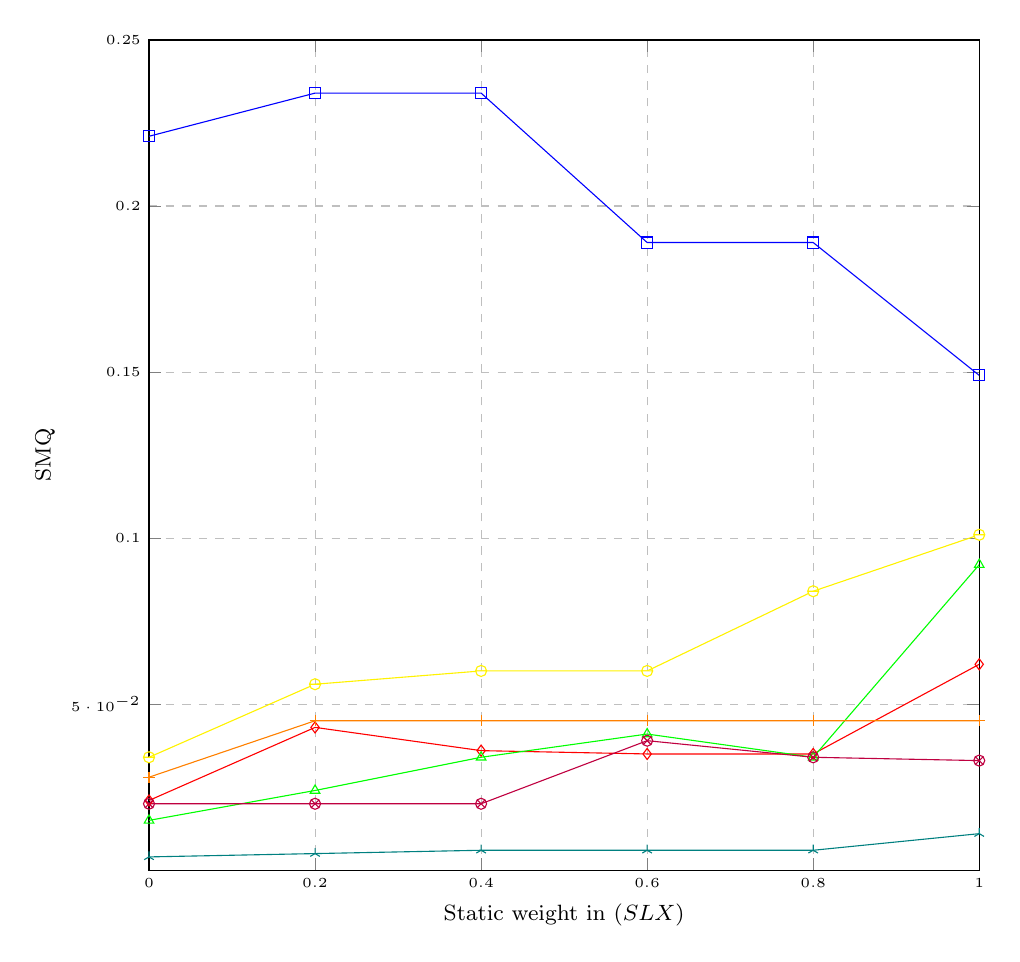
\begin{tikzpicture}
\footnotesize
\begin{axis}[
    width=1.0\textwidth,
    height=1.0\textwidth,
    title={},
    xlabel={Static weight in ($SLX$)},
    ylabel={SMQ},
    xmin=0, xmax=1,
    ymin=0, ymax=0.25,
    xtick={0,0.2,0.4,0.6,0.8,1},
    ytick={0.05,0.1,0.15,0.2,0.25,0.3},
    legend columns=-1,
    legend entries={PyPetstore, Twitter, ChatterBot, asreview, Beets, Picard, Mu},
    legend to name=named,
    ymajorgrids=true,
    xmajorgrids=true,
    grid style=dashed,
    ticklabel style = {font=\tiny}
]

% PyPetstore
\addplot[
    color=blue,
    mark=square,
    ]
    coordinates {
    (0,0.221)(0.2,0.234)(0.4,0.234)(0.6,0.189)(0.8,0.189)(1,0.149)
    };

% Twitter
\addplot[
    color=red,
    mark=diamond,
    ]
    coordinates {
    (0,0.021)(0.2,0.043)(0.4,0.036)(0.6,0.035)(0.8,0.035)(1,0.062)
    };
    
% ChatterBot
\addplot[
    color=green,
    mark=triangle,
    ]
    coordinates {
    (0,0.015)(0.2,0.024)(0.4,0.034)(0.6,0.041)(0.8,0.034)(1,0.092)
    };

% asreview
\addplot[
    color=purple,
    mark=otimes,
    ]
    coordinates {
    (0,0.02)(0.2,0.02)(0.4,0.02)(0.6,0.039)(0.8,0.034)(1,0.033)
    };  

% Beets
\addplot[
    color=orange,
    mark=+,
    ]
    coordinates {
    (0,0.028)(0.2,0.045)(0.4,0.045)(0.6,0.045)(0.8,0.045)(1,0.045)
    };

% Picard
\addplot[
    color=teal,
    mark=Mercedes star,
    ]
    coordinates {
    (0,0.004)(0.2,0.005)(0.4,0.006)(0.6,0.006)(0.8,0.006)(1,0.011)
    };

% Mu
\addplot[
    color=yellow,
    mark=halfcircle,
    ]
    coordinates {
    (0,0.034)(0.2,0.056)(0.4,0.06)(0.6,0.06)(0.8,0.084)(1,0.101)
    };
    
\end{axis}
\end{tikzpicture}

% Data

% Y = [0, 0.2, 0.4, 0.6, 0.8, 1]

% Use this to zip them together, where x is e.g. CHD
% print([x for x in zip(x, y)])

% Only static -> only dynamic

% PyPetstore
% CHM: [0.369, 0.369, 0.25, 0.25, 0.333, 0.756]
% CHD: [0.528, 0.528, 0.479, 0.479, 0.417, 0.511]
% SMQ: [0.167, 0.182, 0.211, 0.211, 0.188, 0.125]
% CMQ: [0.086, 0.101, 0.127, 0.127, 0.125, 0.125]

% Twitter
% CHM: [0.667, 0.636, 0.636, 0.5, 0.5, 0.5]
% CHD: [0.704, 0.486, 0.486, 0.293, 0.293, 0.293]
% SMQ: [0.11, 0.133, 0.142, 0.132, 0.132, 0.149]
% CMQ: [0.077, 0.082, 0.09, 0.097, 0.097, 0.114]

% ChatterBot
% CHM: [0.673, 0.549, 0.563, 0.559, 0.559, 0.752]
% CHD: [0.517, 0.412, 0.463, 0.463, 0.463, 0.767]
% SMQ: [0.138, 0.099, 0.149, 0.148, 0.148, 0.19]
% CMQ: [0.03, 0.02, 0.027, 0.027, 0.027, 0,027, 0.044]

% asreview
% CHM: [0.696, 0.656, 0.672, 0.707, 0.795, 0.747]
% CHD: [0.599, 0.618, 0.616, 0.665, 0.765, 0.73]
% SMQ: [0.175, 0.195, 0.197, 0.192, 0.18, 0.179]
% CMQ: [0.054, 0.127, 0.13, 0.132, 0.115, 0.169]

% Beets
% CHM: [0.57, 0.618, 0.604, 0.626, 0.602, 0.627]
% CHD: [0.45, 0.503, 0.51, 0.51, 0.535, 0.461, 0.365]
% SMQ: [0.082, 0.111, 0.128, 0.129, 0.134, 0.152]
% CMQ: [0.045, 0.084, 0.106, 0.107, 0.107, 0.141]

% Picard

% Mu
% CHM: [0.537, 0.737, 0.784, 0.76, 0.77, 0.72]
% CHD: [0.359, 0.472, 0.522, 0.497, 0.518, 0.472]
% SMQ: [0.132, 0.173, 0.154, 0.157, 0.145, 0.154]
% CMQ: [0.032, 0.109, 0.107, 0.104, 0.092, 0.115]
    \end{subfigure}
    \hfill
    \begin{subfigure}{.5\textwidth}
        \centering
        \input{plots/static_semantic_cmq}
    \end{subfigure}
    \hfill
    \begin{subfigure}{.5\textwidth}
        \centering
        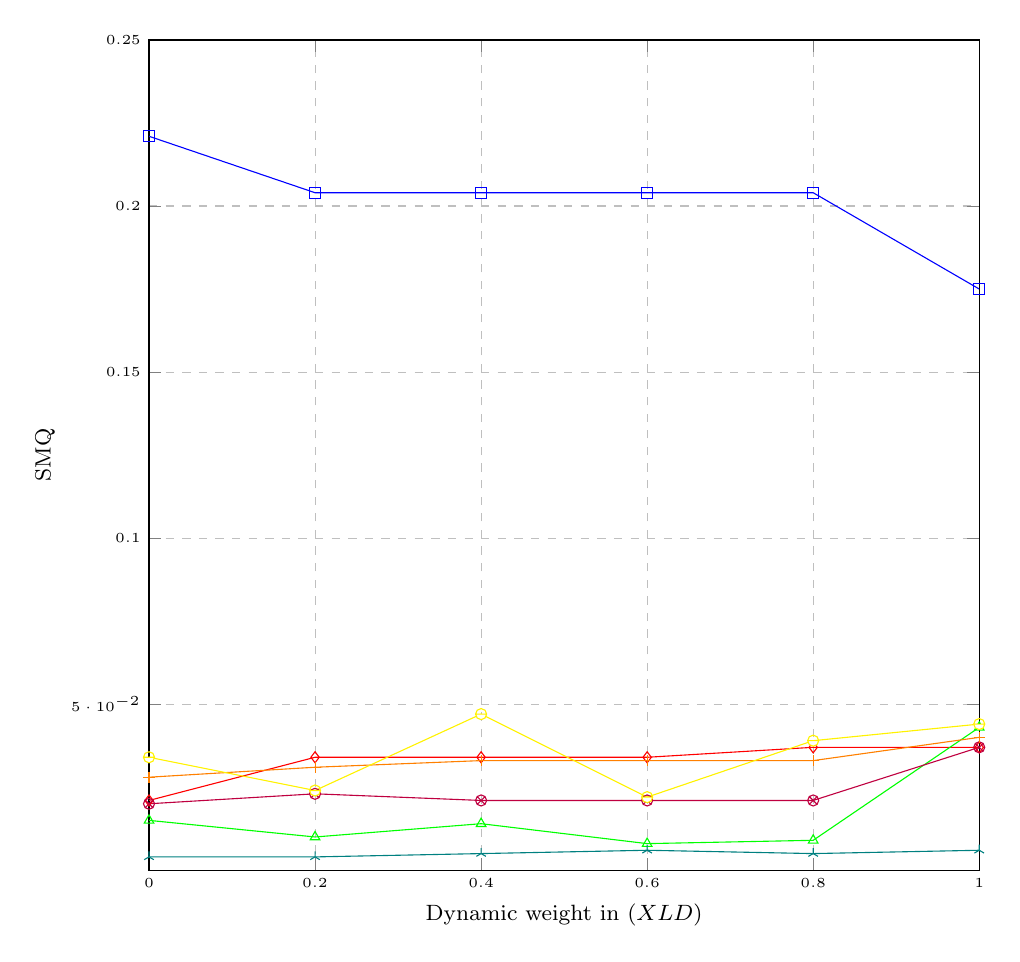
\begin{tikzpicture}
\footnotesize
\begin{axis}[
    width=1.0\textwidth,
    height=1.0\textwidth,
    title={},
    xlabel={Dynamic weight in ($XLD$)},
    ylabel={SMQ},
    xmin=0, xmax=1,
    ymin=0, ymax=0.25,
    xtick={0,0.2,0.4,0.6,0.8,1},
    ytick={0.05,0.1,0.15,0.2,0.25,0.3},
    legend columns=-1,
    legend entries={PyPetstore, Twitter, ChatterBot, asreview, Beets, Picard, Mu},
    legend to name=named,
    ymajorgrids=true,
    xmajorgrids=true,
    grid style=dashed,
    ticklabel style = {font=\tiny}
]

% PyPetstore
\addplot[
    color=blue,
    mark=square,
    ]
    coordinates {
    (0,0.221)(0.2,0.204)(0.4,0.204)(0.6,0.204)(0.8,0.204)(1,0.175)
    };

% Twitter
\addplot[
    color=red,
    mark=diamond,
    ]
    coordinates {
    (0,0.021)(0.2,0.034)(0.4,0.034)(0.6,0.034)(0.8,0.037)(1,0.037)
    };
    
% ChatterBot
\addplot[
    color=green,
    mark=triangle,
    ]
    coordinates {
    (0,0.015)(0.2,0.01)(0.4,0.014)(0.6,0.008)(0.8,0.009)(1,0.043)
    };

% asreview
\addplot[
    color=purple,
    mark=otimes,
    ]
    coordinates {
    (0,0.02)(0.2,0.023)(0.4,0.021)(0.6,0.021)(0.8,0.021)(1,0.037)
    };  

% Beets
\addplot[
    color=orange,
    mark=+,
    ]
    coordinates {
    (0,0.028)(0.2,0.031)(0.4,0.033)(0.6,0.033)(0.8,0.033)(1,0.04)
    };

% Picard
\addplot[
    color=teal,
    mark=Mercedes star,
    ]
    coordinates {
    (0,0.004)(0.2,0.004)(0.4,0.005)(0.6,0.006)(0.8,0.005)(1,0.006)
    };

% Mu
\addplot[
    color=yellow,
    mark=halfcircle,
    ]
    coordinates {
    (0,0.034)(0.2,0.024)(0.4,0.047)(0.6,0.022)(0.8,0.039)(1,0.044)
    };
    \legend{1,2,3,4}
\end{axis}
\end{tikzpicture}

% Data

% Y = [0, 0.2, 0.4, 0.6, 0.8, 1]

% Use this to zip them together, where x is e.g. CHD
% print([x for x in zip(x, y)])

% Only static -> only dynamic

% PyPetstore
% CHM: [0.369, 0.369, 0.25, 0.25, 0.333, 0.756]
% CHD: [0.528, 0.528, 0.479, 0.479, 0.417, 0.511]
% SMQ: [0.167, 0.182, 0.211, 0.211, 0.188, 0.125]
% CMQ: [0.086, 0.101, 0.127, 0.127, 0.125, 0.125]

% Twitter
% CHM: [0.667, 0.636, 0.636, 0.5, 0.5, 0.5]
% CHD: [0.704, 0.486, 0.486, 0.293, 0.293, 0.293]
% SMQ: [0.11, 0.133, 0.142, 0.132, 0.132, 0.149]
% CMQ: [0.077, 0.082, 0.09, 0.097, 0.097, 0.114]

% ChatterBot
% CHM: [0.673, 0.549, 0.563, 0.559, 0.559, 0.752]
% CHD: [0.517, 0.412, 0.463, 0.463, 0.463, 0.767]
% SMQ: [0.138, 0.099, 0.149, 0.148, 0.148, 0.19]
% CMQ: [0.03, 0.02, 0.027, 0.027, 0.027, 0,027, 0.044]

% asreview
% CHM: [0.696, 0.656, 0.672, 0.707, 0.795, 0.747]
% CHD: [0.599, 0.618, 0.616, 0.665, 0.765, 0.73]
% SMQ: [0.175, 0.195, 0.197, 0.192, 0.18, 0.179]
% CMQ: [0.054, 0.127, 0.13, 0.132, 0.115, 0.169]

% Beets
% CHM: [0.57, 0.618, 0.604, 0.626, 0.602, 0.627]
% CHD: [0.45, 0.503, 0.51, 0.51, 0.535, 0.461, 0.365]
% SMQ: [0.082, 0.111, 0.128, 0.129, 0.134, 0.152]
% CMQ: [0.045, 0.084, 0.106, 0.107, 0.107, 0.141]

% Picard

% Mu
% CHM: [0.537, 0.737, 0.784, 0.76, 0.77, 0.72]
% CHD: [0.359, 0.472, 0.522, 0.497, 0.518, 0.472]
% SMQ: [0.132, 0.173, 0.154, 0.157, 0.145, 0.154]
% CMQ: [0.032, 0.109, 0.107, 0.104, 0.092, 0.115]
    \end{subfigure}
    \hfill
    \begin{subfigure}{.5\textwidth}
        \centering
        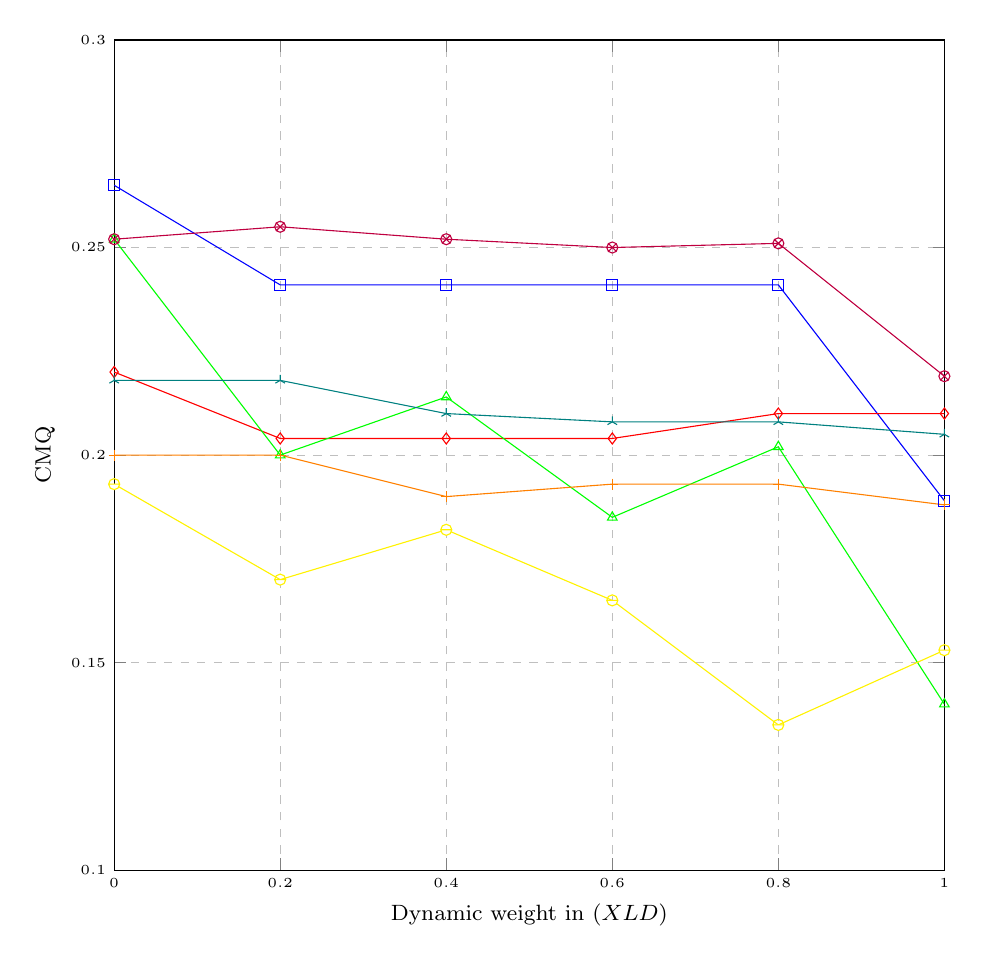
\begin{tikzpicture}
\footnotesize
\begin{axis}[
    width=1.0\textwidth,
    height=1.0\textwidth,
    title={},
    xlabel={Dynamic weight in ($XLD$)},
    ylabel={CMQ},
    xmin=0, xmax=1,
    ymin=0.1, ymax=0.3,
    xtick={0,0.2,0.4,0.6,0.8,1},
    ytick={0.05,0.1,0.15,0.2,0.25,0.3},
    legend columns=-1,
    legend entries={PyPetstore, Twitter, ChatterBot, asreview, Beets, Picard, Mu},
    legend to name=named,
    ymajorgrids=true,
    xmajorgrids=true,
    grid style=dashed,
    ticklabel style = {font=\tiny}
]

% PyPetstore
\addplot[
    color=blue,
    mark=square,
    ]
    coordinates {
    (0,0.265)(0.2,0.241)(0.4,0.241)(0.6,0.241)(0.8,0.241)(1,0.189)
    };

% Twitter
\addplot[
    color=red,
    mark=diamond,
    ]
    coordinates {
    (0,0.22)(0.2,0.204)(0.4,0.204)(0.6,0.204)(0.8,0.21)(1,0.21)
    };
    
% ChatterBot
\addplot[
    color=green,
    mark=triangle,
    ]
    coordinates {
    (0,0.252)(0.2,0.2)(0.4,0.214)(0.6,0.185)(0.8,0.202)(1,0.14)
    };

% asreview
\addplot[
    color=purple,
    mark=otimes,
    ]
    coordinates {
    (0,0.252)(0.2,0.255)(0.4,0.252)(0.6,0.25)(0.8,0.251)(1,0.219)
    };  

% Beets
\addplot[
    color=orange,
    mark=+,
    ]
    coordinates {
    (0,0.2)(0.2,0.2)(0.4,0.19)(0.6,0.193)(0.8,0.193)(1,0.188)
    };

% Picard
\addplot[
    color=teal,
    mark=Mercedes star,
    ]
    coordinates {
    (0,0.218)(0.2,0.218)(0.4,0.21)(0.6,0.208)(0.8,0.208)(1,0.205)
    };

% Mu
\addplot[
    color=yellow,
    mark=halfcircle,
    ]
    coordinates {
    (0,0.193)(0.2,0.17)(0.4,0.182)(0.6,0.165)(0.8,0.135)(1,0.153)
    };
    
\end{axis}
\end{tikzpicture}

% Data

% Y = [0, 0.2, 0.4, 0.6, 0.8, 1]

% Use this to zip them together, where x is e.g. CHD
% print([x for x in zip(x, y)])

% Only static -> only dynamic

% PyPetstore
% CHM: [0.369, 0.369, 0.25, 0.25, 0.333, 0.756]
% CHD: [0.528, 0.528, 0.479, 0.479, 0.417, 0.511]
% SMQ: [0.167, 0.182, 0.211, 0.211, 0.188, 0.125]
% CMQ: [0.086, 0.101, 0.127, 0.127, 0.125, 0.125]

% Twitter
% CHM: [0.667, 0.636, 0.636, 0.5, 0.5, 0.5]
% CHD: [0.704, 0.486, 0.486, 0.293, 0.293, 0.293]
% SMQ: [0.11, 0.133, 0.142, 0.132, 0.132, 0.149]
% CMQ: [0.077, 0.082, 0.09, 0.097, 0.097, 0.114]

% ChatterBot
% CHM: [0.673, 0.549, 0.563, 0.559, 0.559, 0.752]
% CHD: [0.517, 0.412, 0.463, 0.463, 0.463, 0.767]
% SMQ: [0.138, 0.099, 0.149, 0.148, 0.148, 0.19]
% CMQ: [0.03, 0.02, 0.027, 0.027, 0.027, 0,027, 0.044]

% asreview
% CHM: [0.696, 0.656, 0.672, 0.707, 0.795, 0.747]
% CHD: [0.599, 0.618, 0.616, 0.665, 0.765, 0.73]
% SMQ: [0.175, 0.195, 0.197, 0.192, 0.18, 0.179]
% CMQ: [0.054, 0.127, 0.13, 0.132, 0.115, 0.169]

% Beets
% CHM: [0.57, 0.618, 0.604, 0.626, 0.602, 0.627]
% CHD: [0.45, 0.503, 0.51, 0.51, 0.535, 0.461, 0.365]
% SMQ: [0.082, 0.111, 0.128, 0.129, 0.134, 0.152]
% CMQ: [0.045, 0.084, 0.106, 0.107, 0.107, 0.141]

% Picard

% Mu
% CHM: [0.537, 0.737, 0.784, 0.76, 0.77, 0.72]
% CHD: [0.359, 0.472, 0.522, 0.497, 0.518, 0.472]
% SMQ: [0.132, 0.173, 0.154, 0.157, 0.145, 0.154]
% CMQ: [0.032, 0.109, 0.107, 0.104, 0.092, 0.115]
    \end{subfigure}
    \ref{named}
\end{figure}

\paragraph{Coverage}
The coverage is the only metric that follows a clear pattern. The decompositions made with semantic data as input give the highest coverage rate on average (0.971). When combining different graph with each other, the coverage rate increases. As expected, the highest coverage rate is achieved when all information sources are combined. 

\input{tables/results/results_coverage}
% MANUAL: http://ctan.math.washington.edu/tex-archive/graphics/pgf/contrib/tikz-network/tikz-network.pdf

\subsection{Summary}
Table \ref{tab:results_all} gives the mean and standard deviation for each metric applied on the seven different input streams. The grey cell colour indicates the best value obtained for a particular metric. The highest coverage and CHD rates are obtained when incorporating all sources of information ($SLD$). The highest CHM and CMQ rates are achieved when only semantic data is used as input. Decompositions obtained with static information as main source obtain the highest IFN and OPN score. Lastly, the highest SMQ score is achieved for decompositions that combine static and dynamic sources of information.

\begin{table}[h]
    \footnotesize
    \caption{Results of main experiment for all metrics.}\label{tab:results_all}
    \begin{adjustbox}{center}
    \begin{tabular}{>{\raggedright}m{20pt}>{\raggedright}m{45pt}>{\raggedright}m{45pt}>{\raggedright}m{45pt}>{\raggedright}m{50pt}>{\raggedright}m{65pt}>{\raggedright}m{45pt}>{\raggedright\arraybackslash}m{45pt}}
        \toprule
        Input
        & \multicolumn{7}{c}{Metrics}\\
        & Coverage & CHD & CHM & IFN & OPN & SMQ & CMQ \\
        \midrule
        $SXX$ 
        & 0.651$\pm$0.10 & 0.544$\pm$0.14 & 0.643$\pm$0.21 & \cellcolor{CellGray}3.056$\pm$1.42 & \cellcolor{CellGray}52.571$\pm$39.72 & 0.152$\pm$0.02 & 0.115$\pm$0.03\\
        $XLX$ 
        & 0.971$\pm$0.03 & 0.598$\pm$0.10 & \cellcolor{CellGray}0.645$\pm$0.18 & 10.258$\pm$11.04 & 135.714$\pm$134.98 & 0.049$\pm$0.07 & \cellcolor{CellGray}0.229$\pm$0.03 \\
        $XXD$ 
        & 0.625$\pm$0.18 & 0.537$\pm$0.10 & 0.587$\pm$0.13 & 3.995$\pm$2.10 & 65.571$\pm$53.70 & 0.141$\pm$0.04 & 0.096$\pm$0.06 \\
        $SXD$ 
        & 0.846$\pm$0.08 & 0.540$\pm$0.13 & 0.574$\pm$0.24 & 3.623$\pm$1.79 & 68.857$\pm$50.39 & \cellcolor{CellGray}0.164$\pm$0.03 & 0.126$\pm$0.05 \\
        $SLX$ 
        & 0.982$\pm$0.03 & 0.615$\pm$0.13 & 0.662$\pm$0.17 & 8.752$\pm$9.05 & 120.0$\pm$117.11 & 0.059$\pm$0.06 & 0.21$\pm$0.03 \\
        $XLD$ 
        & \cellcolor{CellGray}1.000$\pm$0.00 & 0.591$\pm$0.09 & 0.626$\pm$0.17 & 9.308$\pm$8.19 & 131.714$\pm$127.29 & 0.047$\pm$0.06 & 0.207$\pm$0.030 \\
        $SLD$ 
        & \cellcolor{CellGray}1.000$\pm$0.00 & \cellcolor{CellGray}0.624$\pm$0.12 & 0.643$\pm$0.20 & 9.212$\pm$9.67 & 106.286$\pm$97.75 & 0.059$\pm$0.06 & 0.204$\pm$0.04 \\
        \bottomrule
    \end{tabular}
    \end{adjustbox}
\end{table}

% Projects are alphabetically ordered
% IN: IN1 & IN2 & IN3 & IN4 & IN5 & IN6 & IN7

% M1 PyPetstore
% CHM: 0.756 & 0.305 & 0.369 & 0.250 & 0.667 & 0.250 & 0.250
% CHD: 0.511 & 0.044 & 0.528 & 0.479 & 0.444 & 0.479 & 0.479
% IFN: 1.25 & 4 & 2 & 1.333 & 1 & 1.333 & 1.333
% OPN: 15 & 18 & 19 & 10 & 7 & 10 & 10
% SMQ: 0.125 & -0.094 & 0.167 & 0.211 & 0.146 & 0.211 & 0.211
% CMQ: 0.125 & 0.062 & 0.086 & 0.127 & -0.042 & 0.125 & 0.125
% CF: 0.655 & 0.793 & 0.653 & 0.947 & 0.773 & 0.838 & 0.88
% Coverage: 0.667 & 0.667 & 1 & 0.667 & 1 & 1

% M2 twitter
% CHM: 0.293 & 0.721 & 0.704 & 0.486 & 0.755 & 0.772 & 0.766
% CHD: 0.5 & 0.661 & 0.667 & 0.636 & 0.789 & 0.745 & 0.773
% IFN: 2 & 3.625 & 4.5 & 3.667 & 2.714 & 3.875 & 3.667
% OPN: 20 & 53 & 16 & 26 & 32 & 49 & 37
% SMQ: 0.149 & 0.022 & 0.11 & 0.142 & 0.052 & 0.041 & 0.052
% CMQ: 0.114 & 0.198 & 0.077 & 0.09 & 0.176 & 0.207 & 0.146
% CF: 0.684 & 0.774 & 0.628 & 0.561 & 0.744 & 0.881 & 0.871
% Coverage: 0.615 & 0.910 & 0.423 & 0.756 & 0.962 & 0.987 & 0.987

% M3 ChatterBot
% CHM: 0.752 & 0.516 & 0.673 & 0.563 & 0.568 & 0.489 & 0.561
% CHD: 0.767 & 0.409 & 0.517 & 0.463 & 0.529 & 0.408 & 0.513
% IFN: 2.5 & 4 & 2.25 & 2.857 & 3.5 & 4.6 & 4
% OPN: 28 & 46 & 20 & 43 & 48 & 58 & 42
% SMQ: 0.190 & 0.030 & 0.138 & 0.149 & 0.069 & 0.038 & 0.050
% CMQ: 0.044 & 0.233 & 0.030 & 0.027 & 0.126 & 0.136 & 0.108
% Coverage: 0.449 & 0.878 & 0.653 & 0.714 & 0.898 & 0.959 & 0.980

% M4 asreview
% CHM: 0.747 & 0.668 & 0.696 & 0.707 & 0.725 & 0.669 & 0.661
% CHD: 0.730 & 0.612 & 0.599 & 0.665 & 0.685 & 0.627 & 0.630
% IFN: 4.5 & 9.6 & 4.833 & 4.125 & 7.8 & 8.333 & 8.8
% OPN: 55 & 112 & 73 & 81 & 80 & 113 & 90
% SMQ: 0.179 & 0.033 & 0.175 & 0.192 & 0.038 & 0.034 & 0.039
% CMQ: 0.169 & 0.224 & 0.054 & 0.133 & 0.223 & 0.203 & 0.15
% Coverage: 0.732 & 0.961 & 0.661 & 0.913 & 0.984 & 0.992 & 1

% M5 beets
% CHM: 0.627 & 0.653 & 0.570 & 0.604 & 0.649 & 0.644 & 0.622
% CHD: 0.365 & 0.527 & 0.450 & 0.510 & 0.528 & 0.514 & 0.481
% IFN: 4.667 & 14.8 & 7.167 & 6.667 & 12.667 & 14.4 & 12.167
% OPN: 100 & 234 & 162 & 127 & 238 & 215 & 225
% SMQ: 0.152 & 0.02 & 0.082 & 0.128 & 0.022 & 0.023 & 0.03
% CMQ: 0.141 & 0.165 & 0.045 & 0.106 & 0.173 & 0.167 & 0.167
% Coverage: 0.645 & 1 & 0.671 & 0.865 & 1 & 1 & 1

% M6 picard

% M7 mu
% CHM: 0.720 & 0.699 & 0.537 & 0.802 & 0.737 & 0.739 & 0.782
% CHD: 0.472 & 0.564 & 0.359 & 0.584 & 0.517 & 0.624 & 0.546
% IFN: 2.143 & 8.8 & 2.4 & 2.556 & 4.4 & 6.667 & 3.8
% OPN: 44 & 121 & 30 & 58 & 55 & 87 & 48
% SMQ: 0.154 & 0.021 & 0.132 & 0.157 & 0.084 & 0.036 & 0.085
% CMQ: 0.115 & 0.119 & 0.032 & 0.097 & 0.110 & 0.124 & 0.111
% Coverage: 0.733 & 0.933 & 0.544 & 0.833 & 0.944 & 0.989 & 1


% Data per group (experiment) for statistical test

% PICARD NOT YET INCLUDED
% CHD
% ex1: 0.511, 0.5, 0.767, 0.730, 0.365, 0.472
% ex2: 0.044, 0.661, 0.409, 0.612, 0.527, 0.564
% ex3: 0.528, 0.667, 0.517, 0.599, 0.450, 0.359
% ex4: 0.479, 0.636, 0.463, 0.665, 0.510, 0.584
% ex5: 0.444, 0.789, 0.529, 0.685, 0.528, 0.517
% ex6: 0.479, 0.745, 0.408, 0.627, 0.514, 0.624
% ex7: 0.479, 0.773, 0.513, 0.630, 0.481, 0.546
